\documentclass{article}
\usepackage[utf8]{inputenc}
\usepackage{datetime}
\usepackage{enumerate}
\usepackage{textcomp}
\usepackage{amsmath}
\usepackage{amssymb}
\usepackage{tikz}
\usetikzlibrary{arrows,shapes,backgrounds}

\usepackage{titlesec}
\newcommand{\sectionbreak}{\clearpage}

\title{\bf \Large ASSIGNMENT 3}
\author{Xinhao Luo} 
\date{\today}

\def\math#1{$#1$}

\setlength{\textheight}{8.5in}
\setlength{\textwidth}{6.5in}
\setlength{\oddsidemargin}{0in}
\setlength{\evensidemargin}{0in}
\voffset0.0in

\begin{document}
\maketitle
\medskip

\section{Problem 5.10(j)}

\begin{itemize}
    \item [Claim: ] \math{P(n)} as for \math{n \in \mathbb{N}}, 3 divides \math{n^3 + 5n + 6}.
    \item [Base Case: ] Claim that \math{P(1)} is true; \math{1 + 5 + 6 = 12}; \math{3} divides \math{12}, which is true
    \item [Induction Step: ] Show \math{P(n) \to P(n+1)}, Using direct proof 
        \begin{enumerate}[i)]
            \item Assume \math{P(n)} is true
            \item \begin{equation}
                        \begin{split}
                            (n+1)^3 + 5(n+1) + 6 & = n^3 + 3n^2 + 3n + 1 + 5n + 5 + 6 \\
                            & = n^3 + 3n^2 + 8n + 12 \\
                            & = (n^3 + 5n + 6) + (3n^2 + 3n + 6) \\
                            & = (n^3 + 5n + 6) + 3(n^2 + n + 2)
                        \end{split}
                    \end{equation}
            \item Since 3 divides \math{n^3 + 5n + 6} and \math{3(n^2 + n + 2)}, \math{P(n+1)} is true
            \item \math{P(n) \to P(n+1)} is true
    \end{enumerate}
\end{itemize}

By Induction, \math{P(n)} is true for \math{n \in \mathbb{N}} \math{\hfill{\blacksquare}}

\section{Problem 5.12(i)}

\begin{itemize}
    \item [Claim: ] \math{P(n)} as for \math{n \geq 1}, \math{n! \geq n^n{e}^{-n}}, 
    \item [Base Case: ] Claim that \math{P(1)} is true; \math{1 \geq e^{-1}}, \math{P(1)} is true
    \item [Induction Step: ] Show \math{P(n) \to P(n+1)}, Using direct proof 
        \begin{enumerate}[i)]
            \item Assume \math{P(n)} is true
            \item \begin{equation}
                    \begin{split}
                                n! & \geq n^n{e}^{-n}      \\
                                n!(n+1) & \geq n^n{e}^{-n}(n+1) \\
                                (n+1)!  & \geq n^n{e}^{-n}(n+1) \\
                                (n+1)!  & \geq n^n{e}^{-n-1}(n+1)(1+\frac{1}{n})^n \text{\footnotesize{(derived from hint)}} \\
                                (n+1)!  & \geq (n+1)^n{e}^{-n-1}(n+1) \\
                                (n+1)!  & \geq (n+1)^{(n+1)}{e}^{-n-1} \\
                        \end{split}
                \end{equation}
            \item \math{P(n) \to P(n+1)} is true
        \end{enumerate}
\end{itemize}

By Induction, \math{P(n)} is true for \math{n \geq 1} \math{\hfill{\blacksquare}}

\section{Problem 5.18(a)}

\begin{itemize}
    \item [Claim: ] \math{P(n)} as for \math{H_1 + H_2 + ... + H_n = (n+1)H_n-n}, 
    \item [Base Case: ] Claim that \math{P(1)} is true; \math{1 = (1+1)*1-1}, \math{P(1)} is true
    \item [Induction Step: ] Show \math{P(n) \to P(n+1)}, Using direct proof 
        \begin{enumerate}[i)]
            \item Assume \math{P(n)} is true
            \item \begin{equation}
                    \begin{split}
                                H_1 + H_2 + ... + H_n + H_{n+1} & = H_{n+1} + (n+1)H_n-n      \\
                                & = H_{n+1} + (n+1)(H_{n+1} - \frac{1}{n+1}) - n \\
                                & = H_{n+1} + (n+1)(H_n+1) - 1 - n \\
                                & = (n+2) H_{n+1} - 1 - n
                        \end{split}
                \end{equation}
            \item \math{P(n) \to P(n+1)} is true
        \end{enumerate} 
\end{itemize}

By Induction, \math{P(n)} is true for \math{n \geq 1} \math{\hfill{\blacksquare}}

\section{Problem 5.60}

\begin{enumerate}[(a)]
    \item The perimeter highlighted by the thick line is \math{42}
    \item Prove by induction
        \begin{itemize}
            \item [Claim: ] Perimeter is even for all \math{n \geq 1}
            \item [Base Case: ] \math{P(1)} is true since \math{4} is an even number
            \item [Induction Step: ] Show \math{P(n) \to P(n+1)}, Using direct proof 
                \begin{enumerate}[i)]
                    \item Assume \math{P(n)} is true, the perimeter will be an even number
                    \item there are 5 cases when a new square is added
                    \begin{enumerate}[(1)]
                        \item None side is blocked by the existing squares: the perimeter will \math{+4} under such condition. An even number \math{+4} is still an even number
                        \item One side of the square is blocked by the existing squares: the perimeter will \math{+2}. An even number \math{+2} is still an even number
                        \item Two sides of the square are blocked by the existing squares: The perimeter stays the same, which stays an even number
                        \item Three sides of the square are blocked by the existing squares: The perimeter will be \math{-2}. An even number \math{-2} stays an even number
                        \item Four sides of the square are blocked by the existing squares: the perimeter will \math{-4}. An even number \math{-4} stays an even number.
                        \item \math{P(n) \to P(n+1)} is true
                    \end{enumerate}
                \end{enumerate}
        \end{itemize}
        By Induction, \math{P(n)} is true  \math{\hfill{\blacksquare}}
\end{enumerate}

\section{Problem 6.6}

\begin{enumerate}[(a)]
    \item Proof. \ \begin{itemize}
            \item [Claim: ] \math{P(n)} as for \math{\frac{H_1}{1} + \frac{H_2}{2} + ... + \frac{H_n}{n} \leq \frac{1}{2}{H_n}^2 + 1}, 
            \item [Base Case: ] Claim that \math{P(1)} is true; \math{\frac{1}{1} \leq \frac{1}{2}1^2+1}, \math{P(1)} is true
            \item [Induction Step: ] Show \math{P(1)\land P(2)\land ... \land P(n) \to P(n+1)}, Using direct proof 
                \begin{enumerate}[i)]
                    \item Assume \math{P(1)\land P(2)\land ... \land P(n)} is true
                    \item \begin{equation}
                            \begin{split}
                                        \frac{H_1}{1} + \frac{H_2}{2} + ... + \frac{H_n}{n} & \leq \frac{1}{2}{H_n}^2 + 1 \\
                                        \frac{H_1}{1} + \frac{H_2}{2} + ... + \frac{H_n}{n} + \frac{H_{n+1}}{n+1} & \leq \frac{1}{2}{H_n}^2 + 1 + \frac{H_{n+1}}{n+1} \\
                                        & = \frac{1}{2}{H_n}^2 + 1 + \frac{H_n}{n+1} + \frac{1}{{(n+1)}^2} \\
                                        & = \frac{1}{2}{H_n}^2 + \frac{H_n}{n+1} + \frac{1}{{(n+1)}^2}+ 1 \\
                                        & = \frac{1}{2}({H_n}^2 + \frac{2H_n}{n+1} + \frac{1}{{(n+1)}^2}) + \frac{1}{2{(n+1)}^2} + 1 \\
                                        & = \frac{1}{2}{(H_n + \frac{1}{n+1})}^2 + \frac{1}{2{(n+1)}^2} + 1 \\ 
                                        & = \frac{1}{2}{H_{n+1}}^2 + \frac{1}{2{(n+1)}^2} + 1
                                \end{split}
                        \end{equation}
                    \item \math{\frac{1}{2}{H_{n+1}}^2 + 1 \leq \frac{1}{2}{H_{n+1}}^2 + \frac{1}{2{(n+1)}^2} + 1}
                    \item \math{P(1)\land P(2)\land ... \land P(n) \to P(n+1)} is true
                \end{enumerate} 
        \end{itemize}
        By Induction, \math{P(n)} is true  \math{\hfill{\blacksquare}}
            \item Proof. \ 
                \begin{itemize}
                \item [Claim: ] \math{P(n)} as for \math{\frac{H_1}{1} + \frac{H_2}{2} + ... + \frac{H_n}{n} \leq \frac{1}{2}{H_n}^2 + \frac{1}{2}(\frac{1}{1^2}+\frac{1}{2^2}+...+\frac{1}{n^2})}, 
                \item [Base Case: ] Claim that \math{P(1)} is true; \math{\frac{1}{1} \leq \frac{1}{2}1^2+1}, \math{P(1)} is true
                \item [Induction Step: ] Show \math{P(1)\land P(2)\land ... \land P(n) \to P(n+1)}, Using direct proof 
                    \begin{enumerate}[i)]
                        \item Assume \math{P(1)\land P(2)\land ... \land P(n)} is true
                        \item \begin{equation}
                                \begin{split}
                                            \frac{H_1}{1} + \frac{H_2}{2} + ... + \frac{H_n}{n} & \leq \frac{1}{2}{H_n}^2 + \frac{1}{2}(\frac{1}{1^2}+\frac{1}{2^2}+...+\frac{1}{n^2}) \\
                                            \frac{H_1}{1} + \frac{H_2}{2} + ... + \frac{H_n}{n} + \frac{H_{n+1}}{n+1} & \leq \frac{1}{2}{H_n}^2 + \frac{H_{n+1}}{n+1} + \frac{1}{2}(\frac{1}{1^2}+\frac{1}{2^2}+...+\frac{1}{n^2}) \\
                                            & = \frac{1}{2}{H_n}^2 + \frac{H_n}{n+1} + \frac{1}{{(n+1)}^2} + \frac{1}{2}(\frac{1}{1^2}+\frac{1}{2^2}+...+\frac{1}{n^2})\\
                                            & = \frac{1}{2}{H_n}^2 + \frac{H_n}{n+1} + \frac{1}{{(n+1)}^2} + \frac{1}{2}(\frac{1}{1^2}+\frac{1}{2^2}+...+\frac{1}{n^2})\\
                                            & = \frac{1}{2}({H_n}^2 + \frac{2H_n}{n+1} + \frac{1}{{(n+1)}^2}) + \frac{1}{2{(n+1)}^2} + \frac{1}{2}(\frac{1}{1^2}+\frac{1}{2^2}+...+\frac{1}{n^2}) \\ 
                                            & = \frac{1}{2}{(H_n + \frac{1}{n+1})}^2 + \frac{1}{2{(n+1)}^2} + \frac{1}{2}(\frac{1}{1^2}+\frac{1}{2^2}+...+\frac{1}{n^2}) \\ 
                                            & = \frac{1}{2}{H_{n+1}}^2 + \frac{1}{2}(\frac{1}{1^2}+\frac{1}{2^2}+...+\frac{1}{n^2} + \frac{1}{{(n+1)}^2})
                                    \end{split}
                            \end{equation}
                        \item \math{P(1)\land P(2)\land ... \land P(n) \to P(n+1)} is true
                    \end{enumerate} 
            \end{itemize}
            By Induction, \math{P(n)} is true \math{\hfill{\blacksquare}}
            \item The second claim is stronger since it has narrower scope than the first one.
\end{enumerate}

\section{Problem 6.45(a)}

\begin{itemize}
    \item [Claim: ] \math{P(n)} as There is one special city can be reached by every other city either directly or via one stop.
    \item [Base Case: ] There are three city, and each of them has a one way flight, \math{P(3)} is true as there is always a city can be reached from the others \\
        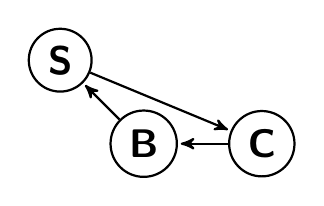
\begin{tikzpicture}[->,>=stealth',shorten >=1pt,auto,node distance=1.5cm,
                        thick,main node/.style={circle,draw,font=\sffamily\Large\bfseries}]
        
          \node[main node] (1) {S};
          \node[main node] (2) [below right of=1] {B};
          \node[main node] (3) [right of=2] {C};

          \path[every node/.style={font=\sffamily\small}]
           (1) edge node [bend right] {} (3)
           (2) edge node [right] {} (1)
           (3) edge node [right] {} (2);
        \end{tikzpicture}
    \item [Induction Step: ] Show \math{P(3) \land P(4) \land ... P(n) \to P(n+1)}, Using direct proof 
        \begin{enumerate}[i)]
            \item Assume \math{P(3) \land P(4) \land ... P(n)} is true
            \item There are three cases. In each cases, \math{B_1, B_2, ...} city and \math{C_1, C_2, ...} have their own connection between each other other than the special city \math{\mathbf{S}}
                \begin{itemize}
                    \item [Case 1] \math{P(n+1)} city has direct flight to current special city. \\ 
                       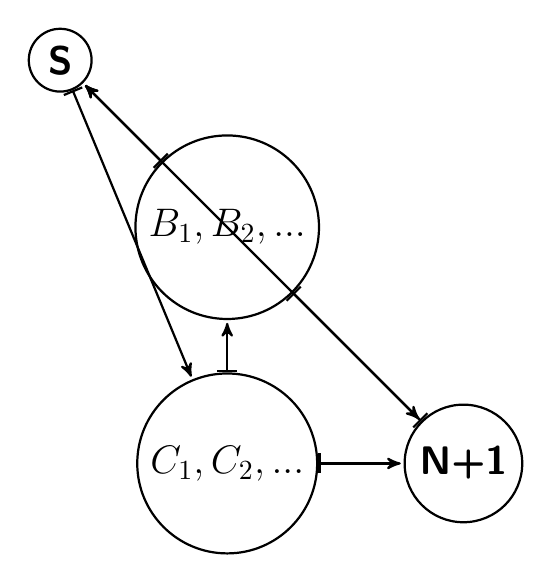
\begin{tikzpicture}[|->,>=stealth',shorten >=1pt,auto,node distance=3cm,
                            thick,main node/.style={circle,draw,font=\sffamily\Large\bfseries}]
            
                          \node[main node] (1) {S};
                          \node[main node] (2) [below right of=1] {\math{B_1, B_2, ...}};
                          \node[main node] (3) [below of=2] {\math{C_1, C_2, ...}};
                          \node[main node] (4) [right of=3] {N+1};
                          
                
                          \path[every node/.style={font=\sffamily\small}]
                           (1) edge node [bend left] {} (3)
                           (2) edge node [right] {} (1)
                           (3) edge node [right] {} (2)
                           (3) edge node [bend left] {} (4)
                           (2) edge node [right] {} (4)
                            (4) edge node [bend left] {} (1);
                        \end{tikzpicture} \\ 
                        The new city will be the same as \math{\mathbf{B}} series cities.
                    \item [Case 2] \math{P(n+1)} city has indirect flight to current special city. \\ 
                       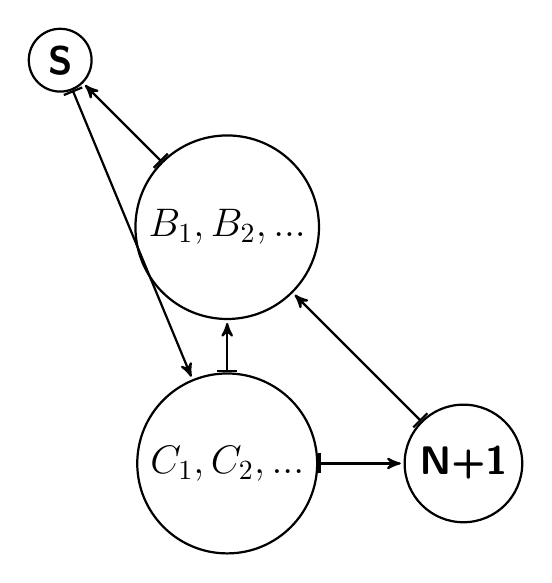
\begin{tikzpicture}[|->,>=stealth',shorten >=1pt,auto,node distance=3cm,
                            thick,main node/.style={circle,draw,font=\sffamily\Large\bfseries}]
            
                          \node[main node] (1) {S};
                          \node[main node] (2) [below right of=1] {\math{B_1, B_2, ...}};
                          \node[main node] (3) [below of=2] {\math{C_1, C_2, ...}};
                          \node[main node] (4) [right of=3] {N+1};
                          
                
                          \path[every node/.style={font=\sffamily\small}]
                           (1) edge node [bend left] {} (3)
                           (2) edge node [right] {} (1)
                           (3) edge node [right] {} (2)
                           (3) edge node [right] {} (4)
                            (4) edge node [bend left] {} (2);
                        \end{tikzpicture} \\ 
                        The new city will be the same as \math{\mathbf{C}} series cities.
                    \item [Case 3] \math{P(n+1)} city has been connected by other cities \\ 
                       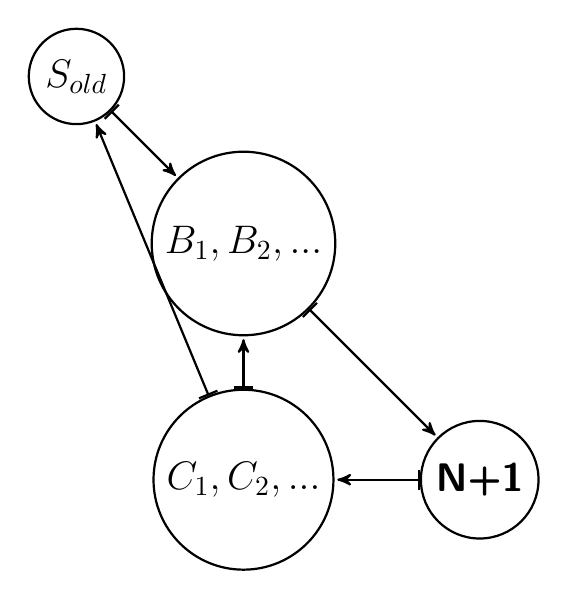
\begin{tikzpicture}[|->,>=stealth',shorten >=1pt,auto,node distance=3cm,
                            thick,main node/.style={circle,draw,font=\sffamily\Large\bfseries}]
            
                          \node[main node] (1) {\math{S_{old}}};
                          \node[main node] (2) [below right of=1] {\math{B_1, B_2, ...}};
                          \node[main node] (3) [below of=2] {\math{C_1, C_2, ...}};
                          \node[main node] (4) [right of=3] {N+1};
                          
                
                          \path[every node/.style={font=\sffamily\small}]
                           (1) edge node [bend left] {} (2)
                           (3) edge node [right] {} (1)
                           (2) edge node [right] {} (4)
                           (3) edge node [right] {} (2)
                            (4) edge node [bend left] {} (3);
                        \end{tikzpicture} \\ 
                        The new city will become the special city.
                \end{itemize}
            \item \math{P(n) \to P(n+1)} is true
    \end{enumerate}
    By Induction, \math{P(n)} is true  \math{\hfill{\blacksquare}}
\end{itemize}

\end{document}
